\SourcePage{689}{692}
\section{Resonance scattering of charged particles}

When charged nuclear particles are scattered (for example, protons by
protons), the short-range nuclear forces are accompanied by the slowly
decreasing Coulomb interaction. The theory of resonance scattering is then
constructed by the same method as in \S~133. The only difference is that,
outside the range of the nuclear forces ($r\gg a$), the exact general solution
of the Schrödinger equation in a Coulomb field must be used in place of the
free-motion solution (133.2). The particle speed is still assumed small only
to the extent that $ka\ll1$; the relation between $1/k$ and the Coulomb unit
of length $a_c=\hbar^2/(mZ_1Z_2e^2)$, where $m$ is the reduced mass of the
colliding particles, may be arbitrary\footnote{The theory presented below was
developed by L.~D.~Landau and Ya.~A.~Smorodinsky (1944).}.

\SourcePage{690}{693}
For motion with $l=0$ in a repulsive Coulomb field, the Schrödinger equation
for the radial function $\chi=rR_0$ is
\begin{equation}
 \chi''+\left(k^2-\frac2r\right)\chi=0
 \tag{138.1}
\end{equation}
(Coulomb units are used here). In \S~36 a solution of this equation was found
subject to the requirement that $\chi/r$ remain finite at $r=0$. Denote this
solution here by $F_0$; it has the form (see (36.27), (36.28))
\begin{equation}
 F_0=Ae^{ikr}krF\left(\frac{i}{k}+1,2,-2ikr\right),\qquad
 A^2=\frac{2\pi/k}{e^{2\pi/k}-1}.
 \tag{138.2}
\end{equation}
Its asymptotic expression at large distances is
\begin{equation}
 F_0\approx\sin\left[kr-\frac1k\ln(2kr)+\delta_0^{\mathrm C}\right],\qquad
 \delta_0^{\mathrm C}=\arg\Gamma\left(1+\frac{i}{k}\right),
 \tag{138.3}
\end{equation}
and the first terms of its expansion at small $r$ ($kr\ll1$, $r\ll1$) are
\begin{equation}
 F_0=Akr(1+r+\ldots).
 \tag{138.4}
\end{equation}
With the changed boundary condition, however, the behavior of the function at
the origin is immaterial, and we need the general solution of (138.1), a
linear combination of its two independent integrals.

The parameters of the confluent hypergeometric function in (138.2), including
the integral value $\gamma=2$, put us precisely in the case mentioned at the
end of \S~d of the Mathematical Supplements. Following the instructions
given there, a second integral of (138.1) is obtained by replacing $F$ in
(138.2) by another linear combination of the two terms whose sum gives the
confluent hypergeometric function according to (d.14). Choosing the difference
of these terms gives the second independent solution of (138.1), denoted by
$G_0$:\footnote{The functions $F_0$ and $G_0$, and the similarly defined
functions $F_l$ and $G_l$ for $l\ne0$, are called the \emph{regular} and
\emph{irregular Coulomb functions}, respectively.}
\begin{equation}
 G_0=2\operatorname{Im}\frac{Ae^{-ikr}kr}{\Gamma(1+i/k)}(-2ikr)^{-1+i/k}
 G\left(1-\frac{i}{k},-\frac{i}{k},-2ikr\right)
 \tag{138.5}
\end{equation}
(the function $F_0$ is the real part of the expression occurring here). Its
asymptotic form at large distances is
\begin{equation}
 G_0\approx\cos\left(kr-\frac1k\ln2kr+\delta_0^{\mathrm C}\right),
 \tag{138.6}
\end{equation}

\SourcePage{691}{694}
and the first terms of the expansion at small $r$ are
\begin{equation}
 G_0=\frac1A\{1+2r[\ln2r+2C-1+h(k)]+\ldots\},
 \tag{138.7}
\end{equation}
where $C=0.577\ldots$ is Euler's constant and $h(k)$ denotes the function
\begin{equation}
 h(k)=\operatorname{Re}\psi\left(-\frac{i}{k}\right)+\ln k
 \tag{138.8}
\end{equation}
(where $\psi(z)=\Gamma'(z)/\Gamma(z)$ is the logarithmic derivative of the
$\Gamma$-function)\footnote{The expansion (138.7) follows from (138.5) by use
of (d.17). The familiar relation
\[
 \psi(1+z)=\psi(z)+\frac1z,
\]
which follows readily from $\Gamma(z+1)=z\Gamma(z)$, and the values
$\psi(1)=-C$, $\psi(2)=-C+1$ have been used.}.

Write the general integral of (138.1) as
\begin{equation}
 \chi=\mathrm{const}\cdot(F_0\cot\delta_0+G_0),
 \tag{138.9}
\end{equation}
where $\cot\delta_0$ is a constant. This notation is chosen so that the
asymptotic form of the solution is
\begin{equation}
 \chi\sim\sin\left[kr-\frac1k\ln(2kr)+\delta_0^{\mathrm C}+\delta_0\right].
 \tag{138.10}
\end{equation}
Thus $\delta_0$ is the additional shift of the wave-function phase caused by
the short-range forces. It must be related to the constant in the boundary
condition $(\chi'/\chi)|_{r\to0}=\mathrm{const}$ which replaces consideration
of the wave function within the range of the nuclear forces. Because the
logarithmic derivative $\chi'/\chi$ diverges as $\ln r$ when $r\to0$, this
condition must now be imposed not at zero but at an arbitrarily small, yet
finite, value $r=\rho$. Calculating $\chi'(\rho)/\chi(\rho)$ from (138.4) and
(138.7) and equating it to a constant gives
\[
 kA^2\cot\delta_0+2[\ln2\rho+2C+h(k)]=\mathrm{const}.
\]
The left-hand side contains the $k$-independent constants
$2\ln2\rho+4C$; include them in the constant and then denote it by
$-\kappa$. The final expression for $\cot\delta_0$, now in ordinary units,
is
\begin{equation}
 \cot\delta_0=-\frac1\pi(e^{2\pi/ka_c}-1)
 \left[h(ka_c)+\frac{\kappa a_c}{2}\right].
 \tag{138.11}
\end{equation}

\SourcePage{692}{695}
In the limit $1/a_c\to0$, corresponding to uncharged particles, (138.11)
becomes $\cot\delta_0=-\kappa/k$, in agreement with (133.6). Figure~49 shows
the function $h(x)$\footnote{The function $h(k)$ may be calculated from
\[
 h(k)=k^{-2}\sum_{n=1}^{\infty}\frac1{n(n^2+k^{-2})}-C+\ln k,
\]
which follows readily from
\[
 \psi(z)=-C-\frac1z+z\sum_{n=1}^{\infty}\frac1{n(n+z)}
\]
(see E.~Whittaker and G.~Watson, \emph{A Course of Modern Analysis}, Vol.~II,
\S~12.16; Moscow: Fizmatgiz, 1963). The limiting expressions for $h(k)$ are
\[
 h(k)\approx\frac{k^2}{12}\quad\text{for }k\ll1,\qquad
 h(k)=-C+\ln k+\frac{1.2}{k^2}\quad\text{for }k\gg1
\]
(the latter gives values of $h(k)$ with an error below $4\%$ already for
$k>2.5$).}.

\begin{figure}[htbp]
\centering
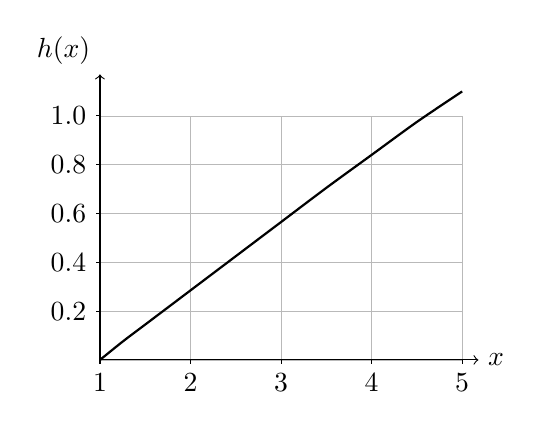
\begin{tikzpicture}[x=1.15cm,y=3.1cm]
  \draw[xstep=1,ystep=.2,gray!55,very thin] (1,0) grid (5,1);
  \draw[->] (1,0) -- (5.18,0) node[right] {$x$};
  \draw[->] (1,0) -- (1,1.17) node[above left] {$h(x)$};
  \foreach \x in {1,2,3,4,5} \draw (\x,0) -- ++(0,-0.018) node[below] {\x};
  \foreach \y/\lab in {0.2/{0.2},0.4/{0.4},0.6/{0.6},0.8/{0.8},1.0/{1.0}}
    \draw (1,\y) -- ++(-0.045,0) node[left] {\lab};
  \draw[thick] plot[smooth] coordinates {
    (1,0.00) (1.25,0.075) (1.5,0.145) (1.75,0.215)
    (2,0.285) (2.5,0.425) (3,0.565) (3.5,0.705)
    (4,0.84) (4.5,0.975) (5,1.10)};
\end{tikzpicture}
\caption{The function $h(x)$.}
\end{figure}

Thus, in the presence of the Coulomb interaction, the following quantity is
``constant'':
\begin{equation}
 \frac{2\pi\cot\delta_0}{a(e^{2\pi/ka_c}-1)}
 +\frac2{a_c}h(ka_c)=-\kappa.
 \tag{138.12}
\end{equation}
We have put the word ``constant'' in quotation marks because $\kappa$ is actually the first term in the expansion, in powers of the small quantity $ka$, of a certain function that depends on the properties of the short-range forces. As noted in \S~133, a resonance at low energies corresponds to an anomalously small value of the constant $\kappa$. Greater accuracy therefore requires retaining the next term of the expansion ($\sim k^2$), whose coefficient has a ``normal'' order of magnitude; that is, $-\kappa$ in (138.12) must be replaced by\footnote{For proton--proton scattering, the constants $a=1/\kappa_0$ and $r_0$ have the values $a=-7.8\cdot10^{-13}$, $r_0=2.8\cdot10^{-13}$ cm (the Coulomb unit of length is $2\hbar^2/m_pe^2=57.6\cdot10^{-13}$ cm). These values refer to a proton pair with antiparallel spins (when the spins are parallel, the Pauli principle prevents the two-proton system from occupying an $s$ state at all).}

\[
 -\kappa_0+\frac12r_0k^2.
\]

The presence of a resonance may be associated, as noted in \S~133, with either an actual or a virtual\SourcePage{693}{696}
discrete bound state of the system. One can show\footnote{See L.~D.~Landau and Ya.~A.~Smorodinsky, ZhETF, vol.~14 (1944), p.~269.} that the sign of the constant $\kappa$ remains the criterion for deciding whether the level is actual or virtual.


According to (138.10), the full phase shifts of the wave functions are
$\delta_l^{\mathrm C}+\delta_l$. Therefore the scattering cross-section is
\begin{equation}
 f(\theta)=\frac1{2ik}\sum_{l=0}^{\infty}(2l+1)
 [\exp(2i\delta_l^{\mathrm C}+2i\delta_l)-1]P_l(\cos\theta).
 \tag{138.13}
\end{equation}
Write the difference in square brackets as
\begin{align}
 \exp(2i\delta_l^{\mathrm C}+2i\delta_l)-1
 ={}&[\exp(2i\delta_l^{\mathrm C})-1]\notag\\
 &+[\exp(2i\delta_l^{\mathrm C})(e^{2i\delta_l}-1)].
 \tag{138.14}
\end{align}
The Coulomb phases $\delta_l^{\mathrm C}$ make contributions of the same
order to the scattering amplitude for every $l$. The phases $\delta_l$
associated with the short-range forces, however, are small for $l\ne0$ at
low energies. Thus, on substituting (138.14) in (138.13), retain the first
bracket in every term of the sum; these terms sum to the Coulomb scattering
amplitude (135.9),
\begin{equation}
 f_{\mathrm C}(\theta)=-\frac1{2a_ck^2\sin^2(\theta/2)}
 \exp\left(-\frac{2i}{ka_c}\ln\sin\frac\theta2+2i\delta_0^{\mathrm C}\right).
 \tag{138.15}
\end{equation}
Retain the second bracket in (138.14) only in the term with $l=0$. The full
scattering amplitude is therefore
\begin{equation}
 f(\theta)=f_{\mathrm C}(\theta)+\frac1{2ik}(e^{2i\delta_0}-1)
 \exp(2i\delta_0^{\mathrm C}).
 \tag{138.16}
\end{equation}

The second term may be called the nuclear scattering amplitude. It must be
emphasized, however, that this separation is conventional. Through the
definition of $\delta_0$ in (138.11), the Coulomb interaction substantially
affects this term too, making it entirely different from what the same
short-range forces would give for uncharged particles. In particular, as
$ka_c\to0$, $\delta_0$, and hence the entire second term in (138.16), tends
exponentially to zero, as $\exp(-2\pi/ka_c)$; nuclear scattering is then
completely masked by Coulomb repulsion.

\SourcePage{694}{697}
The two parts of the amplitude interfere in the scattering cross-section:
\begin{align}
 \frac{d\sigma}{d\Omega}=|f(\theta)|^2
 ={}&\left(\frac{Z_1Z_2e^2}{2mv^2}\right)^2
 \left[\frac1{\sin^4(\theta/2)}\right.\notag\\
 &\left.-\frac{4ka_c}{\sin^2(\theta/2)}\sin\delta_0
 \cos\left(\frac2{ka_c}\ln\sin\frac\theta2+\delta_0\right)
 +4(ka_c)^2\sin^2\delta_0\right].
 \tag{138.17}
\end{align}
Here the colliding particles are assumed distinct. For identical particles,
the scattering amplitude would first have to be symmetrized before its square
is taken (compare \S~137).
